%
% schnittgerade.tex
%
% (c) 2018 Prof Dr Andreas Müller, Hochschule Rapperswil
%
\documentclass[tikz,12pt]{standalone}
\usepackage{times}
\usepackage{amsmath}
\usepackage{txfonts}
\usepackage[utf8]{inputenc}
\usepackage{graphics}
\usetikzlibrary{arrows,intersections,math}
\usepackage{ifthen}
\begin{document}

\newboolean{showgrid}
\setboolean{showgrid}{false}

\begin{tikzpicture}[>=latex,thick]

% Povray Bild
\node at (0,0) {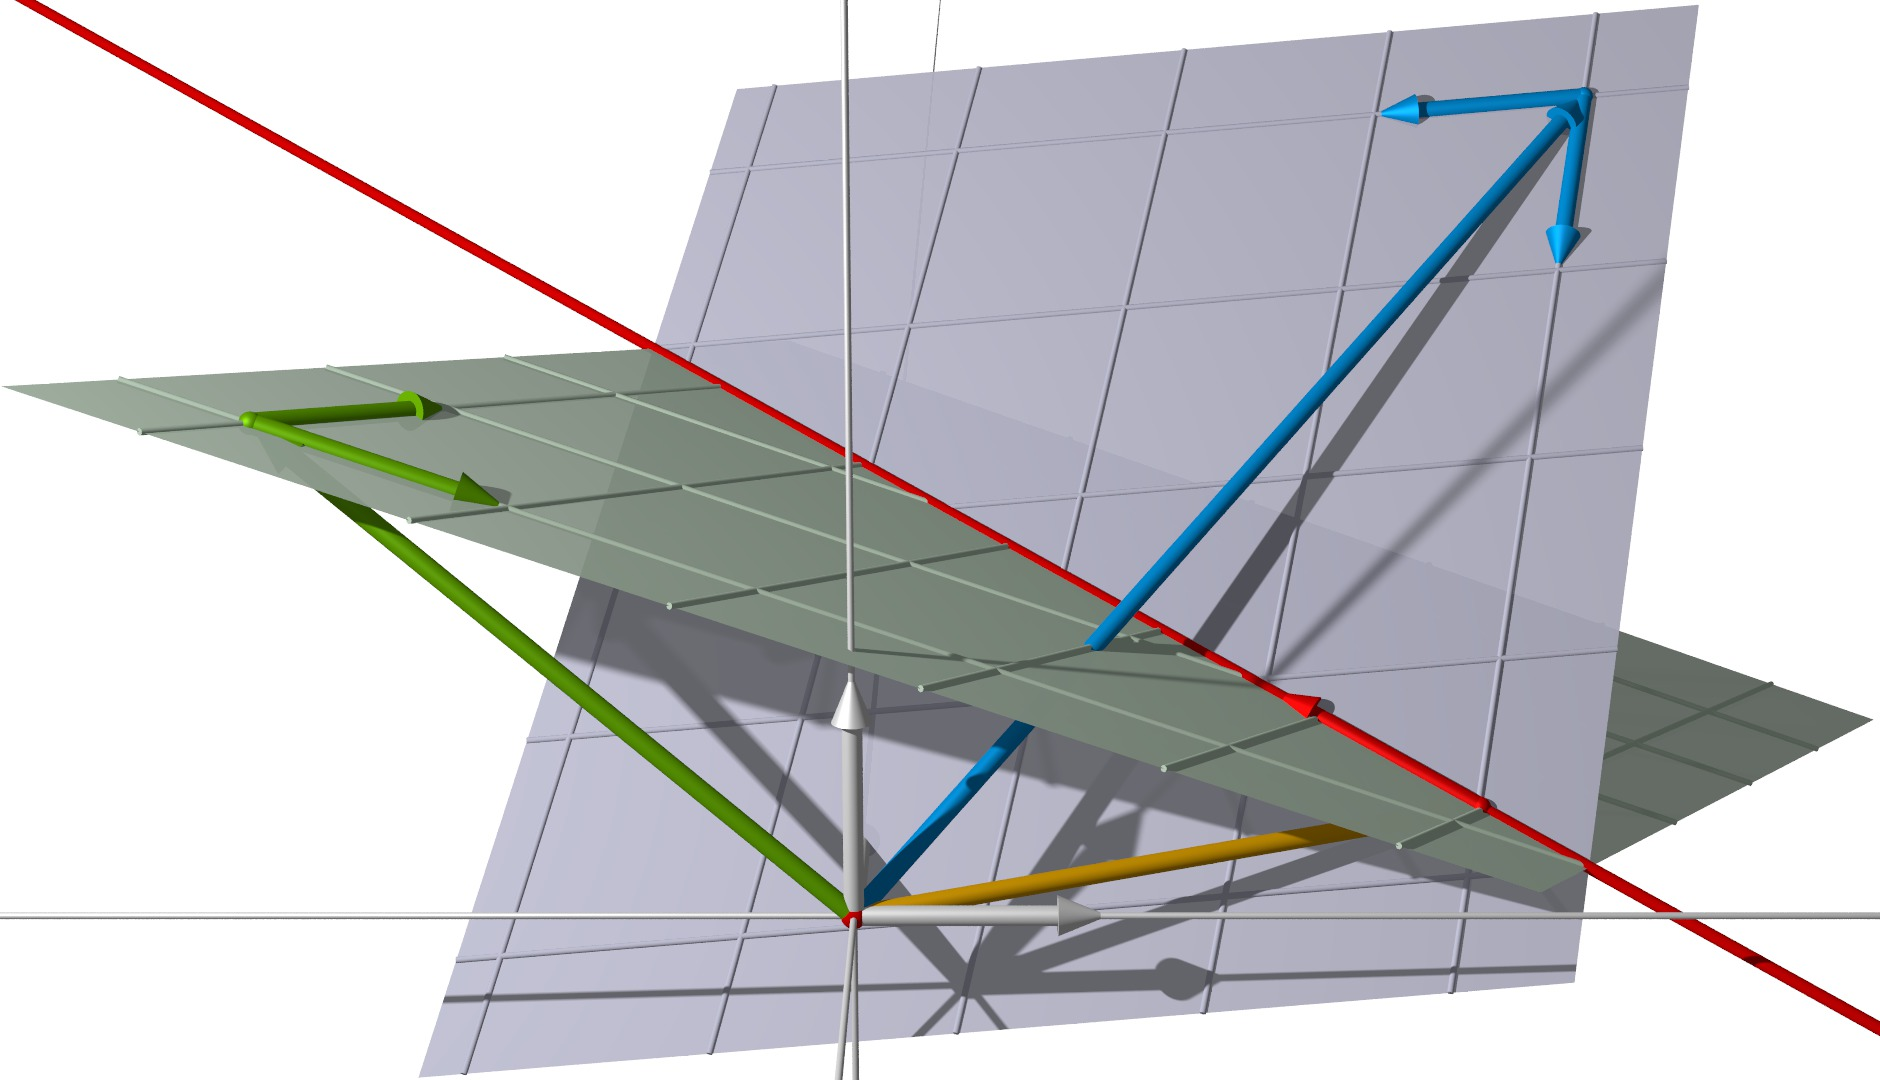
\includegraphics[width=14cm]{schnittgerade.jpg}};

% Gitter
\ifthenelse{\boolean{showgrid}}{
\draw[step=0.1,line width=0.1pt] (-7,-4) grid (7, 4);
\draw[step=0.5,line width=0.4pt] (-7,-4) grid (7, 4);
\draw (-7,-4) grid (7, 4);
\fill (0,0) circle[radius=0.05];
}{}

% grüne Ebene
\node at (-5.2,1.2) {$P_0$};
\node at (-3.2,0.5) {$\vec{u}_0$};
\node at (-3.7,1.3) {$\vec{v}_0$};
\node at (-3.5,-0.9) {$\vec{p}_0$};
\node at (-2,0.1) {$\sigma_0$};

% blaue Ebene
\node at (5,3.5) {$P_1$};
\node at (3.2,3.4) {$\vec{u}_1$};
\node at (4.6,1.8) {$\vec{v}_1$};
\node at (3,1.8) {$\vec{p}_1$};
\node at (-0.2,3.1) {$\sigma_1$};

% Gerade
\node at (2.7,-0.9) {$\vec{r}$};
\node at (4.2,-1.7) {$Q_0$};
\node at (1.7,-2.1) {$\vec{q}_0$};
\node at (-3, 2.2) {$g$};

% Nullpunkt
\node at (-0.9,-3.1) {$O$};

\end{tikzpicture}

\end{document}

